\subsection{Spider evaluation with GPT 3.5 and GPT 4}

Throughout this thesis, we have explored the advancements in Text-to-SQL models and their performance on the SPIDER benchmark. Our analysis revealed the significant progress made in the field, with more recent models demonstrating remarkable improvements in generating accurate SQL queries from natural language text.

The integration of powerful pre-trained language models, such as BERT, and cutting-edge architectures like T5 has played a vital role in the observed advancements. The models' ability to learn from limited labeled data, quickly adapt to new tasks or domains, and handle complex SQL queries has been substantially enhanced by employing techniques such as active learning, meta-learning, and multi-task learning.

Our experiments with ChatGPT-3.5 and ChatGPT-4.0 have showcased their superior performance, achieving scores of 81.30\% and 85.20\% on the SPIDER benchmark, respectively. These results highlight the potential of utilizing the latest huge language models for Text-to-SQL tasks, further pushing the boundaries of what is possible in this domain.

As the field of natural language processing continues to evolve, we can expect even more sophisticated models and techniques to emerge, enabling more accurate and efficient understanding and generation of SQL queries from natural language input. Future research in this area may focus on enhancing the models' ability to handle ambiguous or imprecise input, as well as exploring novel methods to improve their adaptability and generalization capabilities across diverse tasks and domains.

\begin{table}[h]
    \centering
    \begin{tabular}{|c|c|c|c|c|c|}
        \hline
        \multirow{2}*{Exact Match Accuracy} & easy  & medium & hard  & extra hard & all            \\
                                            & 248   & 446    & 174   & 166        & 1034           \\ \hline
        GPT 3.5 execution                   & 0.964 & 0.883  & 0.644 & 0.596      & 0.816          \\ \hline
        GPT 3.5 exact match                 & 0.972 & 0.881  & 0.621 & 0.596      & 0.813          \\ \hline
        GPT 4 execution                     & 0.980 & 0.930  & 0.678 & 0.651      & \textbf{0.855} \\ \hline
        GPT 4 exact match                   & 0.980 & 0.933  & 0.667 & 0.639      & \textbf{0.852} \\ \hline
    \end{tabular}
    \caption{Comparison between Exact Match Accuracy}
\end{table}

In conclusion, our experience using the ChatGPT API for the Text-to-SQL task on the SEOSS dataset was positive. The model's powerful natural language understanding capabilities, combined with the ease of integration through the API, make it a valuable tool for addressing such tasks. Additionally, by incorporating a few values from the database into the system input prompt, ChatGPT can better comprehend the database structure and generate more accurate queries. Also, by including the history of queries in prompts, we can improve the model's accuracy, but it will increase the overall time and money required to generate the queries. Future work could involve further fine-tuning ChatGPT specifically for Text-to-SQL tasks or exploring more advanced techniques for error correction and query validation.

% add SPIDER benchmark diagram image
\begin{figure}[h]
    \centering
    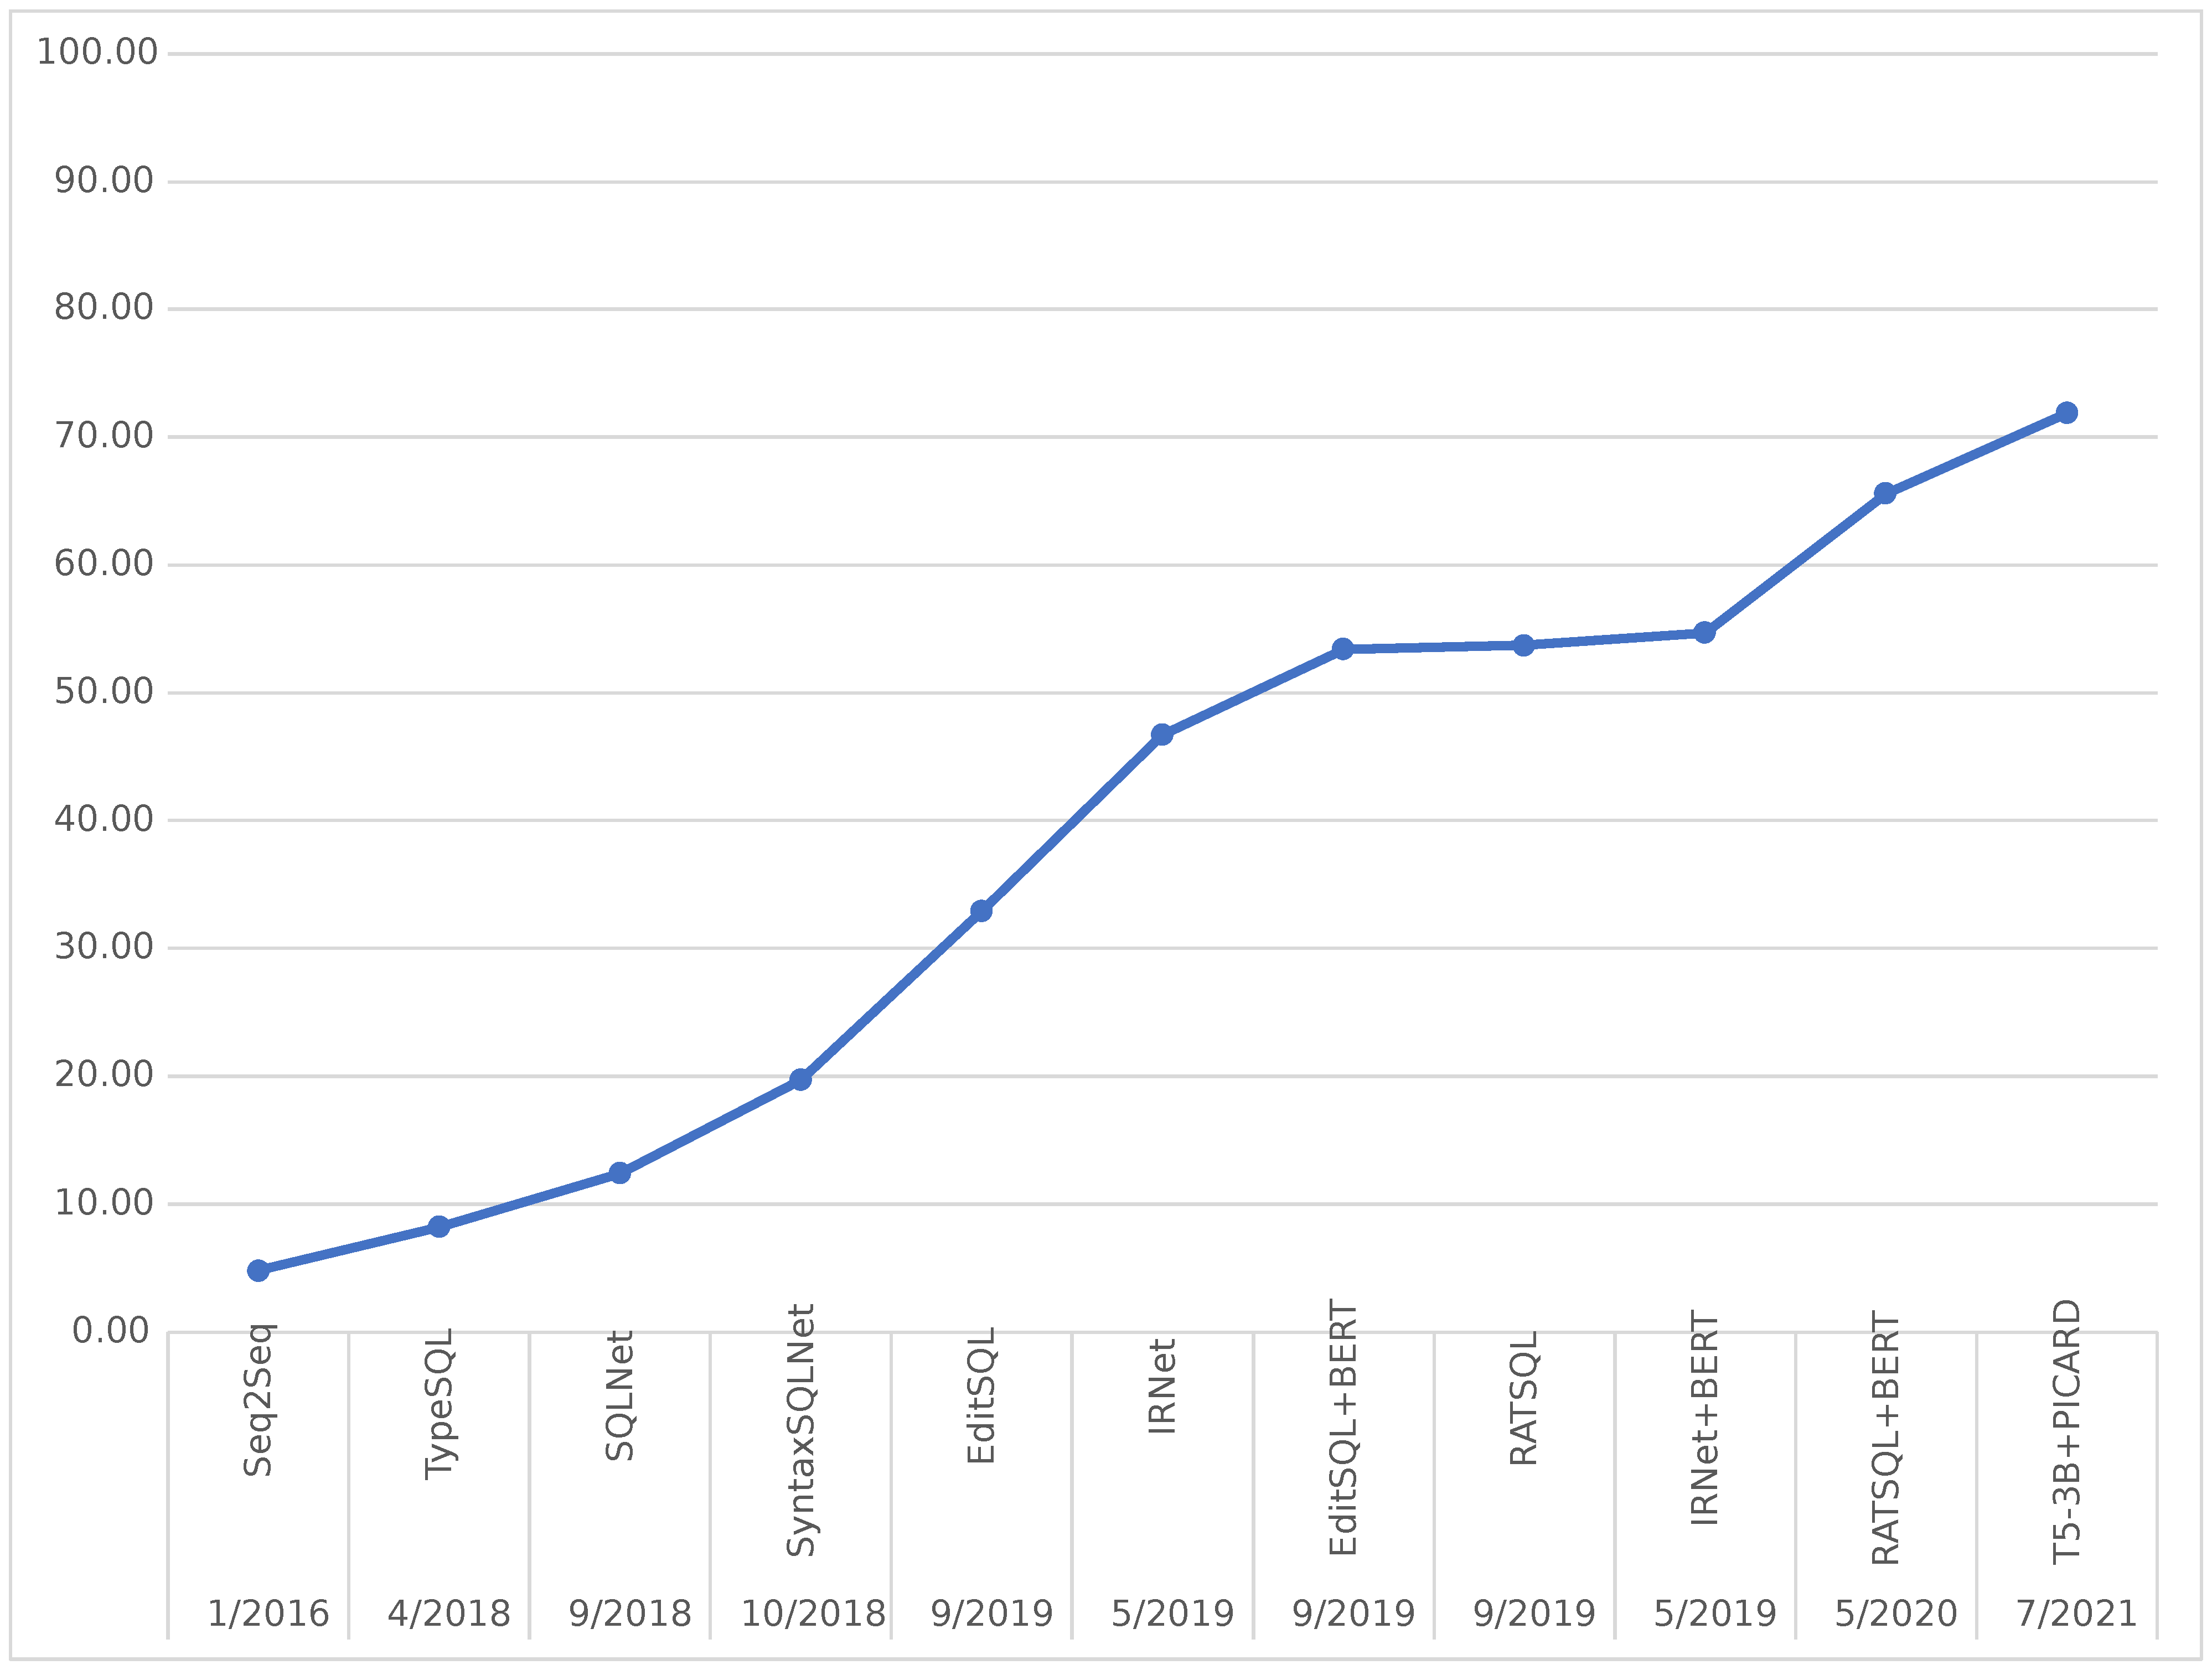
\includegraphics[width=0.99\linewidth]{pics/benchmarkeps}
    \caption{SPIDER benchmark Exact Match Results including our experiments}
    \label{fig:benchmark}
\end{figure}